\documentclass[12pt]{article}
\usepackage{amsmath}  % Math
\usepackage{amssymb}  % Symbols
\usepackage{graphicx} % Images
\usepackage[utf8]{inputenc}
\usepackage[T1]{fontenc}
\usepackage[margin=1in]{geometry}
\usepackage[spanish]{babel}
\usepackage{transparent}
\usepackage{eso-pic}
\usepackage{xcolor}
\usepackage{subcaption} % For subfigures
\usepackage{array} % For thicker table lines and better column definitions
\usepackage{booktabs} % For professional quality tables
\usepackage{longtable} % For tables that span multiple pages
\usepackage{float} % For [H] option in tables/figures
\usepackage{fancyhdr} % For custom headers/footers
\usepackage{longtable} % For tables that can span multiple pages

\graphicspath{{images/}} % Path to images
\newcommand\BackgroundPic{
    \put(0,0){
        \parbox[b][\paperheight]{\paperwidth}{
            \vfill
            \centering
            \transparent{0.1}
\includegraphics[width=\paperwidth]{logo} % your image
            \vfill
        }
    }
}


\title{Informe Negocio Empanadas: \\
\textit{Las Empanadas Hermanas}} % Title of the report
  \author{Autores: Felipe Colli, Juan Gonzalez, Bastián Ortiz y Javier Robles \thanks{Instituto Nacional General José Miguel Carrera} \\
  Curso: \textit{4°H}, Profesor: \textit{Carlos Morales}} % Add your names and course
  \date{30 de mayo de 2025} % Fecha de Entrega
\AddToShipoutPicture{\BackgroundPic} % Add background image

\begin{document}

\maketitle
%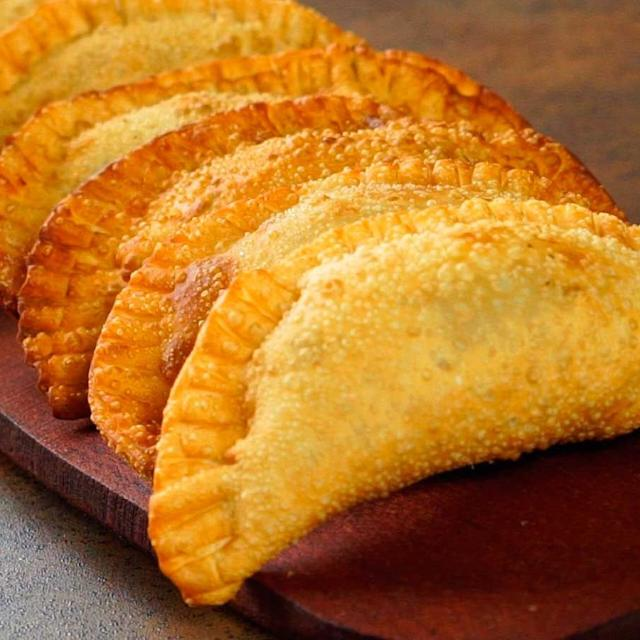
\includegraphics[width=0.95\textwidth]{empanadas} % Logo of the school
\begin{figure}[h]
    \centering
    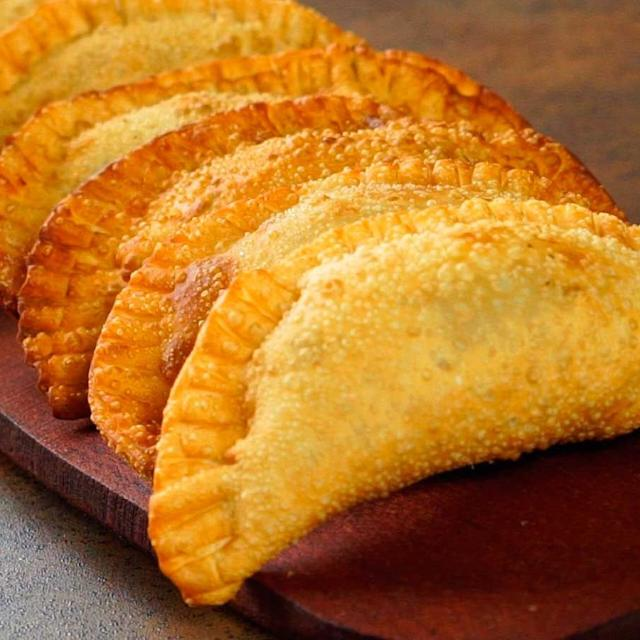
\includegraphics[width=0.85\textwidth]{empanadas} % Logo of the school
\end{figure}
\newpage

\tableofcontents
\newpage

\section{Resumen} % Aprox 1/3 de Pagina
\newpage



\section{Introducción} % Max 1 pagina
El presente informe tiene como objetivo presentar el negocio de empanadas "Las Empanadas Hermanas", un emprendimiento que busca ofrecer empanadas de alta calidad. A través de este documento, se detallarán los aspectos clave del negocio, incluyendo su propuesta de valor, mercado objetivo y proyecciones financieras iniciales correspondientes al primer avance del trabajo de Matemática Financiera. \\

Dentro de las proyecciones financieras, se contempla un análisis de costos y precios para una producción inicial, así como una estimación de las ganancias esperadas. El negocio se enfoca en la producción y venta de tres variedades principales de empanadas: Pino (carne), Queso Clásica, y Camarón Queso, con un énfasis en la calidad de los ingredientes y la satisfacción del cliente. Todo esto se desarrolla sin olvidar el marco legal regulatorio, por lo cual este negocio no será un frente para lavado de activos, evasión de impuestos, generación de facturas ideológicamente falsas, o la venta de drogas ilícitas. \\ % Referencia a Breking Bad y Los Pollos Hermanos. Mantener el toque estudiantil.


\subsection{Objetivos del Negocio:}
\begin{enumerate}
    \item \textbf{Propuesta de Valor Inicial:} Ofrecer tres variedades de empanadas (Pino, Queso, Camarón Queso) de alta calidad, elaboradas con ingredientes frescos, destacando el sabor tradicional.
    \item \textbf{Estimación de Producción y Ventas:} Definir una cantidad inicial de productos a vender para el primer mes (500 unidades por variedad, total 1500 empanadas).
    \item \textbf{Análisis de Costos de Ingredientes:} Cotizar los ingredientes en al menos dos proveedores y seleccionar los más convenientes para elaborar una lista de compras detallada y valorizada.
    \item \textbf{Gestión de IVA en Compras:} Elaborar una factura de compra simulada que refleje el valor neto de los ingredientes, el IVA crédito fiscal y el total pagado.
    \item \textbf{Estrategia de Precios y Proyección de Ingresos:} Definir precios de venta competitivos para cada variedad, que cubran costos y generen ganancia. Calcular el ingreso total neto esperado y el IVA débito fiscal.
    \item \textbf{Cálculo de Obligaciones Tributarias (IVA):} Determinar el monto de IVA a pagar al fisco, resultante de la diferencia entre IVA débito e IVA crédito.
    \item \textbf{Evaluación de Rentabilidad Inicial:} Calcular las ganancias del primer mes y verificar si son suficientes para reinvertir en la producción del mes siguiente y obtener un excedente (sueldo para el grupo).
    \item \textbf{Viabilidad del Negocio (Preliminar):} Evaluar la viabilidad preliminar del negocio basándose en los cálculos financieros del primer mes de operación.

\end{enumerate}

\newpage



\section{Desarrollo} % 2 - 5 paginas
% \subsection{} % This was empty, removed.

\subsection{Tabla de Costos de Ingredientes}

%\begin{table}[H] % Using [H] from float package to place it "here"
    %\centering
    \begin{longtable}{|| c | c | c | c||}
        \hline
        \textbf{Distribuidor} & Formato & \textbf{Costo} &  \\ [0.5ex]
        \hline\hline
        \multicolumn{3}{||c|}{\textbf{Masa Prehecha Grande}} & \textbf{Costo 100 unidades} \\ [0.5ex] \hline \hline
        El Palacio de las Empanadas & 20 Un & \$4100 & \$20500 \\ \hline
        Alimentos La Kosa & 20 Un & \$4200 & \$21000 \\ [1ex] \hline \hline

        \multicolumn{3}{||c|}{\textbf{Huevos}} & \textbf{Costo por Docena} \\ [0.5ex] \hline \hline
        El Don Huevo & 180 Un & \$39500 & \$2633 \\ \hline
        Huevos La Montaña Pelluhue & 180 Un & \$43990 & \$2932 \\ [1ex] \hline

        \multicolumn{3}{||c|}{\textbf{Camaron}} & \textbf{Costo por KG} \\ [0.5ex] \hline \hline
        Distribuidora GK & 10 KG & \$48900 & \$4890 \\ \hline
        Comercial Oceanica & 10 KG & \$55800 & \$5580 \\ [1ex] \hline

        \multicolumn{3}{||c|}{\textbf{Carne Molida}} & \textbf{Costo por KG} \\ [0.5ex] \hline \hline % Added Costo por KG header for consistency
        Central Mayorista & 500 G & \$2590 & \$5080 \\ \hline 
        El Paiquito & 250 G & \$1090 & \$4360 \\ [1ex] \hline \hline


        \multicolumn{3}{||c|}{\textbf{Queso}} & \textbf{Costo por KG} \\ [0.5ex] \hline \hline % Added Costo por KG header
        Distribuidora Santiago & 1 KG & \$9580 & \$9580 \\ \hline
        Distribuidora Nueva de Matte & 1 KG & \$6940 & \$6940 \\ [1ex] \hline

        \multicolumn{3}{||c|}{\textbf{Cebolla}} & \textbf{Costo por KG} \\ [0.5ex] \hline \hline % Added Costo por KG header
        Santiago Natural Foods & 14 KG & \$10990 & \$785 \\ \hline
        Distribuidora Frest & 10 KG & \$9990 & \$990 \\ [1ex] \hline

        \multicolumn{3}{||c|}{\textbf{Aceite}} & \textbf{Costo por Litro} \\ [0.5ex] \hline \hline
        ProsudMarket & 18 L & \$39614 & \$2200.77 \\ \hline
        Central Mayorista & 13.5 L & \$22200 & \$1644.44 \\ [1ex] \hline
        
        \multicolumn{3}{||c|}{\textbf{Sal}} & \textbf{Costo por KG} \\ [0.5ex] \hline \hline % Added Costo por KG header
        Central Mayorista & 10 KG & \$4400 & \$440 \\ \hline
        Distribuidora Online & 1 Kg & \$358 & \$358 \\ [1ex] \hline \hline

        \multicolumn{3}{||c|}{\textbf{Oregano}} & \textbf{Costo por KG} \\ [0.5ex] \hline \hline % Added Costo por KG header
        La Vega & 1 KG & \$3796 & \$3796 \\ \hline
        Santiago Natural Foods & 1 KG & \$6900 & \$6900 \\ [1ex] \hline \hline

        \multicolumn{3}{||c|}{\textbf{Comino}} & \textbf{Costo por KG} \\ [0.5ex] \hline \hline % Added Costo por KG header
        Los Cholitos & 1 KG & \$4284 & \$4284 \\ \hline
        Directo de la Vega & 1 KG & \$5177 & \$5177 \\ [1ex] \hline \hline

        \multicolumn{3}{||c|}{\textbf{Pimienta}} & \textbf{Costo por KG} \\ [0.5ex] \hline \hline % Added Costo por KG header
        Directo de la Vega & 1 KG & \$3106 & \$3106 \\ \hline
        CDV Foods & 1 KG & \$3068 & \$3068 \\ [1ex] \hline \hline

        \multicolumn{3}{||c|}{\textbf{Pasas}} & \textbf{Costo por KG} \\ [0.5ex] \hline \hline % Added Costo por KG header
        Chile Frutos Secos & 1 KG & \$3690 & \$3690 \\ \hline
        Nutri Bueno & 1 KG & \$4000 & \$4000 \\ [1ex] \hline \hline


        \multicolumn{3}{||c|}{\textbf{Aceitunas}} & \textbf{Costo por KG} \\ [0.5ex] \hline \hline % Added Costo por KG header
        Alaia Gourmet & 1 KG & \$4000 & \$4000 \\ \hline
        Mercado Libre & 1 KG & \$4900 & \$4900 \\ [1ex] \hline \hline

    %\end{longtable}
    \caption{Tabla de Costos de Ingredientes por Proveedor}
    \label{tab:costos_ingredientes_proveedor}
    \end{longtable} %n Priemra Pagina del Desarrollo
%\newpage


\subsection{Cotizaciones de Ingredientes}
    %\subsubsection{Masa Prehecha}
        \begin{figure}[H] % Use [H] or [htbp] for better float placement
            \centering % Center the content of the figure
            \begin{subfigure}{0.35\textwidth}
                \centering
                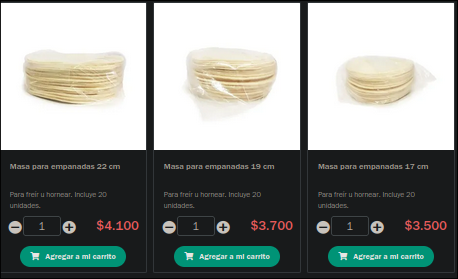
\includegraphics[width=0.9\linewidth]{palaci} % Removed space before ]
                \caption{Palacio de las Empanadas}
                \label{fig:palacio}
            \end{subfigure}
            \hfill % Add some space between subfigures
            \begin{subfigure}{0.35\textwidth}
                \centering
                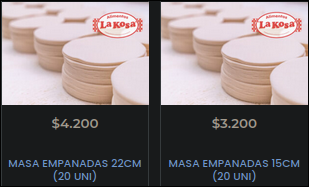
\includegraphics[width=0.9\linewidth]{kosa} % Removed space before ]
                \caption{Alimentos La Kosa}
                \label{fig:kosa}
            \end{subfigure}
            \caption{Cotizaciones de Distribuidores de Masa Prehecha}
            \label{fig:cotizaciones_masas}
        \end{figure} % END OF THIS FIGURE

    %\subsubsection{Huevos}
        \begin{figure}[H] % START A NEW FIGURE
            \centering
            \begin{subfigure}{0.3\textwidth}
                \centering
                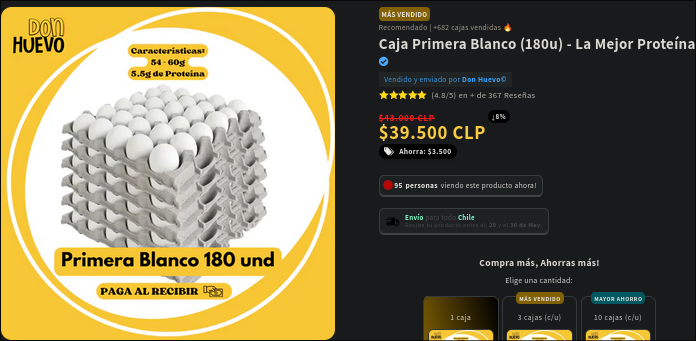
\includegraphics[width=0.9\linewidth]{donhuevo} % Removed space before ]
                \caption{El Don Huevo}
                \label{fig:don_huevo}
            \end{subfigure}
            \hfill
            \begin{subfigure}{0.35\textwidth}
                \centering
                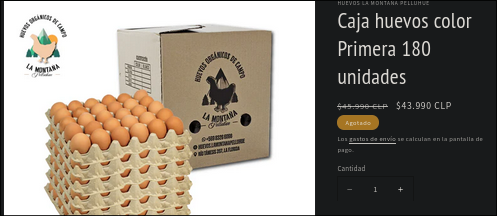
\includegraphics[width=0.9\linewidth]{montan1} % Removed space before ]
                \caption{Huevos La Montaña Pelluhue}
                \label{fig:huevos_montaña}
            \end{subfigure}
            \caption{Cotizaciones de Distribuidores de Huevos}
            \label{fig:cotizaciones_huevos}
        \end{figure} % END OF THIS FIGURE

    %\subsubsection{Camaron}
        \begin{figure}[H] % START A NEW FIGURE
            \centering
            \begin{subfigure}{0.35\textwidth}
                \centering
                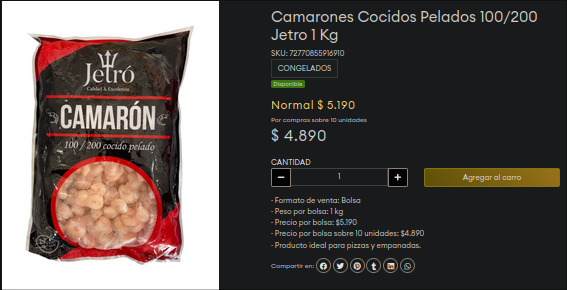
\includegraphics[width=0.9\linewidth]{gk} % Removed space before ]
                \caption{Distribuidora GK}
                \label{fig:distribuidora_gk}
            \end{subfigure}
            \hfill
            \begin{subfigure}{0.3\textwidth}
                \centering
                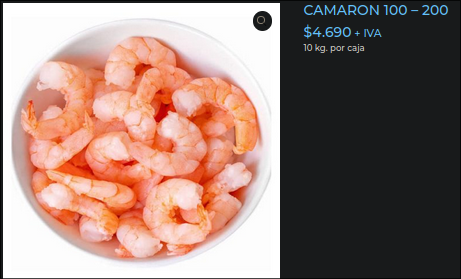
\includegraphics[width=0.9\linewidth]{oceanic} % Removed space before ]
                \caption{Comercial Oceanica}
                \label{fig:comercial_oceanica}
            \end{subfigure}
            \caption{Cotizaciones de Distribuidores de Camarón}
            \label{fig:cotizaciones_camaron}
        \end{figure} % END OF THIS FIGURE
         \newpage 
        % Fin segunda pagina del desarrollo

    %\subsubsection{Carne Molida}
        \begin{figure}[H] % START A NEW FIGURE
            \centering
            \begin{subfigure}{0.35\textwidth}
                \centering
                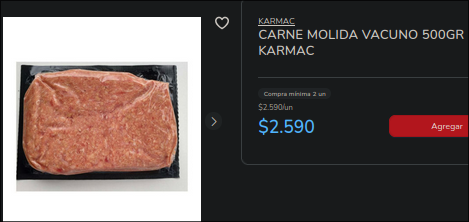
\includegraphics[width=0.9\linewidth]{central} % Removed space before ]
                \caption{Central Mayorista}
                \label{fig:central_mayorista}
            \end{subfigure}
            \hfill
            \begin{subfigure}{0.3\textwidth}
                \centering
                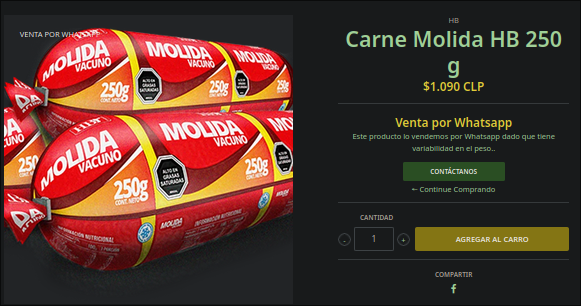
\includegraphics[width=0.9\linewidth]{paiquito} % Removed space before ]
                \caption{Paiquito}
                \label{fig:paiquito} 
            \end{subfigure}
            \caption{Cotizaciones de Distribuidores de Carne Molida}
            \label{fig:cotizaciones_carne_molida}
        \end{figure} % END OF THIS FIGURE

    %\subsubsection{Queso}
        \begin{figure}[H] % START A NEW FIGURE
            \centering
            \begin{subfigure}{0.45\textwidth}
                \centering
                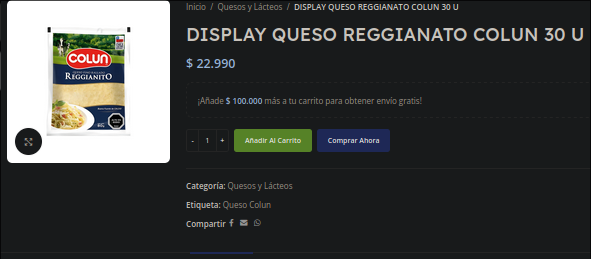
\includegraphics[width=0.9\linewidth]{santiago} % Removed space before ]
                \caption{Distribuidora Santiago}
                \label{fig:distribuidora_santiago}
            \end{subfigure}
            \hfill
            \begin{subfigure}{0.37\textwidth}
                \centering
                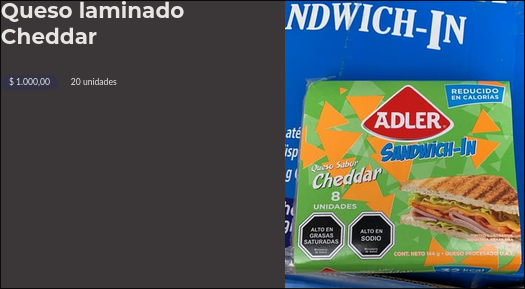
\includegraphics[width=0.9\linewidth]{nueva} % Removed space before ]
                \caption{Distribuidora Nueva de Matte}
                \label{fig:distribuidora_nueva_de_matte}
            \end{subfigure}
            \caption{Cotizaciones de Distribuidores de Queso}
            \label{fig:cotizaciones_queso}
        \end{figure} % END OF THIS FIGURE

    %\subsubsection{Cebolla}
        \begin{figure}[H] % START A NEW FIGURE
            \centering
            \begin{subfigure}{0.4\textwidth}
                \centering
                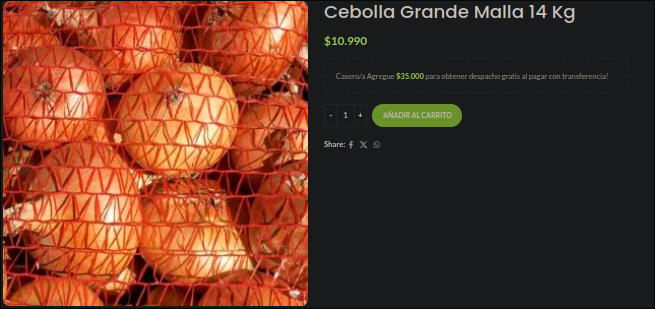
\includegraphics[width=0.9\linewidth]{nat} % Removed space before ]
                \caption{Santiago Natural Foods}
                \label{fig:santiago_natural_foods}
            \end{subfigure}
            \hfill
            \begin{subfigure}{0.45\textwidth}
                \centering
                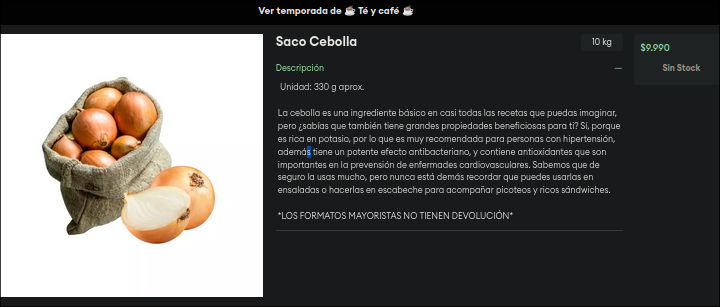
\includegraphics[width=0.9\linewidth]{fres} % Removed space before ]
                \caption{Distribuidora Frest}
                \label{fig:distribuidora_frest}
            \end{subfigure}
            \caption{Cotizaciones de Distribuidores de Cebolla}
            \label{fig:cotizaciones_cebolla}
        \end{figure} % END OF THIS FIGURE

    %\subsubsection{Aceite}
        \begin{figure}[H] % START A NEW FIGURE
            \centering
            \begin{subfigure}{0.45\textwidth}
                \centering
                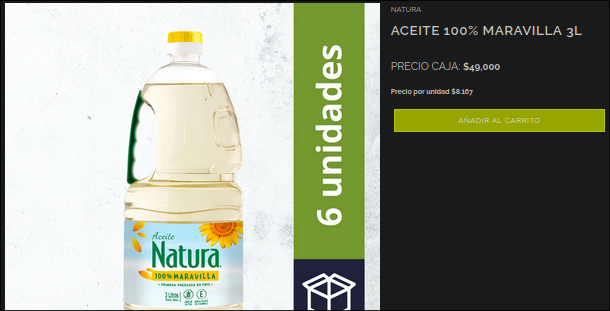
\includegraphics[width=0.9\linewidth]{prosud} % Removed space before ]
                \caption{ProsudMarket}
                \label{fig:prosudmarket}
            \end{subfigure}
            \hfill
            \begin{subfigure}{0.46\textwidth}
                \centering
                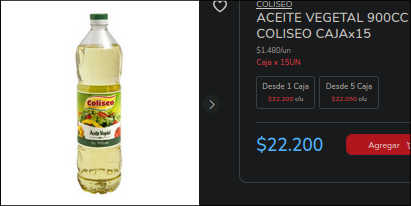
\includegraphics[width=0.9\linewidth]{aceite} % Removed space before ]
                \caption{Central Mayorista}
                \label{fig:central_mayorista_aceite}
            \end{subfigure}
            \caption{Cotizaciones de Distribuidores de Aceite}
            \label{fig:cotizaciones_aceite}
        \end{figure} % END OF THIS FIGURE
        % Fin tercera pagina del desarrollo

    %\subsubsection{Sal}
        \begin{figure}[H] % START A NEW FIGURE
            \centering
            \begin{subfigure}{0.4\textwidth}
                \centering
                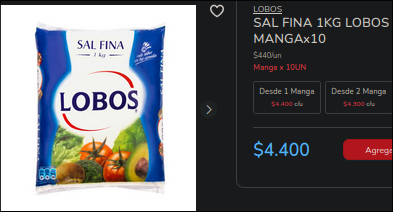
\includegraphics[width=0.9\linewidth]{lobos} % Removed space before ]
                \caption{Central Mayorista}
                \label{fig:central_mayorista_sal}
            \end{subfigure}
            \hfill
            \begin{subfigure}{0.35\textwidth}
                \centering
                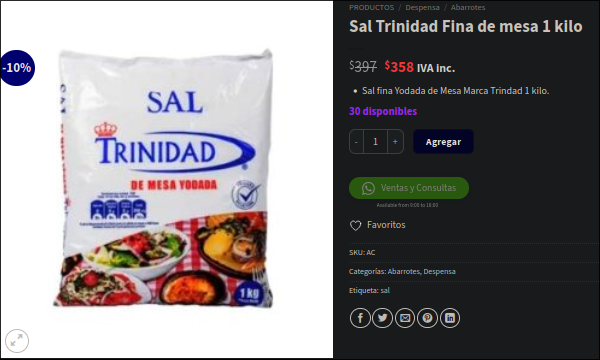
\includegraphics[width=0.9\linewidth]{online} % Removed space before ]
                \caption{Distribuidora Online}
                \label{fig:distribuidora_online_sal}
            \end{subfigure}
            \caption{Cotizaciones de Distribuidores de Sal}
            \label{fig:cotizaciones_sal}
        \end{figure} % END OF THIS FIGURE

    %\subsubsection{Oregano}
        \begin{figure}[H] % START A NEW FIGURE
            \centering
            \begin{subfigure}{0.5\textwidth}
                \centering
                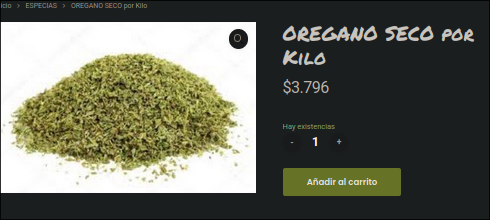
\includegraphics[width=0.9\linewidth]{vega} % Removed space before ]
                \caption{La Vega}
                \label{fig:la_vega_oregano}
            \end{subfigure}
            \hfill
            \begin{subfigure}{0.4\textwidth}
                \centering
                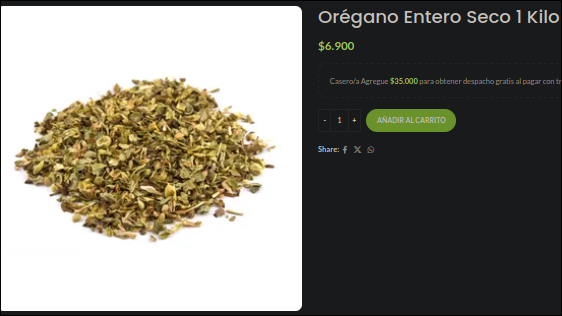
\includegraphics[width=0.9\linewidth]{Oregano} % Removed space before ]
                \caption{Santiago Natural Foods}
                \label{fig:santiago_natural_foods_oregano}
            \end{subfigure}
            \caption{Cotizaciones de Distribuidores de Oregano}
            \label{fig:cotizaciones_oregano}
        \end{figure} % END OF THIS FIGURE

    %\subsubsection{Comino}
        \begin{figure}[H] % START A NEW FIGURE
            \centering
            \begin{subfigure}{0.4\textwidth}
                \centering
                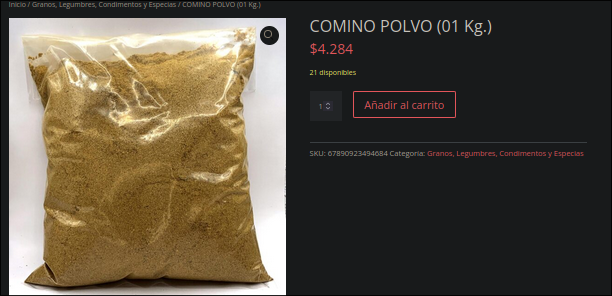
\includegraphics[width=0.9\linewidth]{cholitos} % Removed space before ]
                \caption{Los Cholitos}
                \label{fig:los_cholitos_comino}
            \end{subfigure}
            \hfill
            \begin{subfigure}{0.45\textwidth}
                \centering
                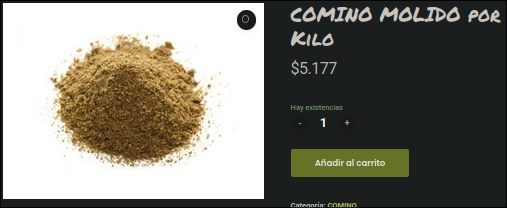
\includegraphics[width=0.9\linewidth]{comino} % Removed space before ]
                \caption{Directo de la Vega}
                \label{fig:directo_de_la_vega_comino}
            \end{subfigure}
            \caption{Cotizaciones de Distribuidores de Comino}
            \label{fig:cotizaciones_comino}
        \end{figure} % END OF THIS FIGURE

    %\subsubsection{Pimienta}
        \begin{figure}[H] % START A NEW FIGURE
            \centering
            \begin{subfigure}{0.45\textwidth}
                \centering
                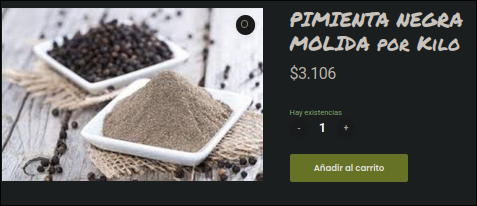
\includegraphics[width=0.9\linewidth]{negra} % Removed space before ]
                \caption{Directo de la Vega}
                \label{fig:directo_de_la_vega_pimienta}
            \end{subfigure}
            \hfill
            \begin{subfigure}{0.5\textwidth}
                \centering
                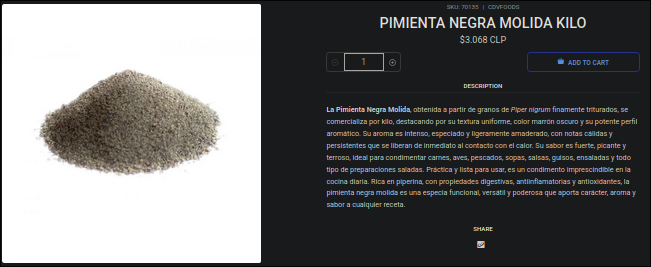
\includegraphics[width=0.9\linewidth]{pimienta} % Removed space before ]
                \caption{CDV Foods}
                \label{fig:cdv_foods_pimienta}
            \end{subfigure}
            \caption{Cotizaciones de Distribuidores de Pimienta}
            \label{fig:cotizaciones_pimienta}
        \end{figure} % END OF THIS FIGURE

    %\subsubsection{Pasas}
        \begin{figure}[H] % START A NEW FIGURE
            \centering
            \begin{subfigure}{0.4\textwidth}
                \centering
                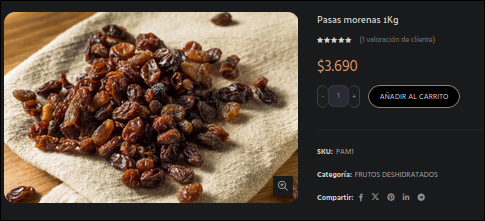
\includegraphics[width=0.9\linewidth]{chile} % Removed space before ]
                \caption{Chile Frutos Secos}
                \label{fig:chile_frutos_secos_pasas}
            \end{subfigure}
            \hfill
            \begin{subfigure}{0.45\textwidth}
                \centering
                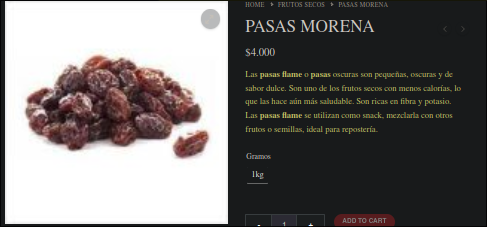
\includegraphics[width=0.9\linewidth]{nutri} % Removed space before ]
                \caption{Nutri Bueno}
                \label{fig:nutri_bueno_pasas}
            \end{subfigure}
            \caption{Cotizaciones de Distribuidores de Pasas}
            \label{fig:cotizaciones_pasas}
        \end{figure} % END OF THIS FIGURE

    %\subsubsection{Aceitunas}
        \begin{figure}[H] % START A NEW FIGURE
            \centering
            \begin{subfigure}{0.45\textwidth}
                \centering
                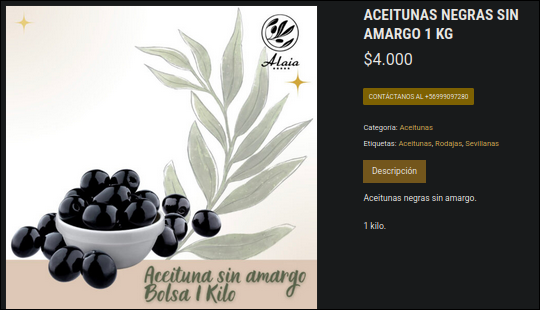
\includegraphics[width=0.9\linewidth]{gourmet} % Removed space before ]
                \caption{Alaia Gourmet}
                \label{fig:alaia_gourmet_aceitunas}
            \end{subfigure}
            \hfill
            \begin{subfigure}{0.4\textwidth}
                \centering
                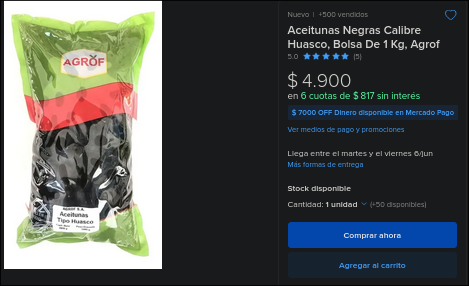
\includegraphics[width=0.9\linewidth]{libre} % Removed space before ]
                \caption{Mercado Libre}
                \label{fig:mercado_libre_aceitunas}
            \end{subfigure}
            \caption{Cotizaciones de Distribuidores de Aceitunas}
            \label{fig:cotizaciones_aceitunas}
        \end{figure} % END OF THIS FIGURE

        
        %\newpage 

    \subsection{Facturas e IVA} 
        \subsubsection{Lista de Compras Detallada y Costos Seleccionados}
        Para la producción inicial de 1500 empanadas (500 de cada variedad: Pino, Queso Clásica, Camarón Queso), se seleccionaron los proveedores con los precios más convenientes para cada ingrediente, según la Tabla \ref{tab:costos_ingredientes_proveedor}. Las cantidades y costos se detallan en la Tabla \ref{tab:lista_compras}.

        \begin{table}[H]
            \centering
            \small % Reduce font size for this table
            \begin{tabular}{|l|l|r|c|r|r|}
                \hline
                \textbf{Ingrediente} & \textbf{Proveedor Elegido} & \textbf{Cantidad} & \textbf{Unidad} & \textbf{Costo Unitario} & \textbf{Costo Total} \\
                \hline
                Masa Prehecha & El Palacio de las Emp. & 1500 & Unidades & \$205 & \$307.500 \\
                Huevos & El Don Huevo & 10 & Docenas & \$2.633 & \$26.400 \\
                Camarón & Del Origen & 40 & KG & \$4.870 & \$194.800 \\
                Carne Molida & El Paiquito & 25 & KG & \$4.360 & \$109.000 \\
                Queso Mantecoso & Dist. Nueva de Matte & 45 & KG & \$6.940 & \$312.300 \\
                Cebolla & Santiago Natural Foods & 42 & KG & \$785 & \$31.500 \\
                Aceite & Central Mayorista & 16 & Litros & \$1.644,44 & \$26.311 \\
                Sal & Central Mayorista & 10 & KG & \$440 & \$4400 \\
                Oregano & La Vega & 1 & KG & \$3.780 & \$3780 \\
                Comino & Los Cholitos & 1 & KG & \$4284 & \$4284 \\
                Pimienta & CDV Foods & 1 & KG & \$3068 & \$3068 \\
                Pasas & Chile Frutos Secos & 1 & KG & \$3690 & \$ 3690 \\
                Aceitunas & Alaia Gourmet & 3 & KG & \$4000 & \$12000 \\
                \hline
                \multicolumn{5}{|r|}{\textbf{TOTAL NETO COMPRAS}} & \textbf{\$} \\
                \hline
            \end{tabular}
            \caption{Lista de Compras para 1500 Empanadas.}
            \label{tab:lista_compras}
        \end{table}

        \subsubsection{Factura de Compra}
    \subsection{Definición de Precios y Proyección de Ingresos}
        \subsubsection{Costos Unitarios y Precios de Venta}
        \subsubsection{Proyección de Ingresos y Cálculo de IVA}
        \subsubsection{Cálculo de Ganancias y Viabilidad Inicial}
        \newpage
   
\section{Conclusiones} % Max 1 pagina


\end{document}

